\documentclass[uct_visualisation_thesis.tex]{subfiles}

\section{Wykorzystane technologie}
W naszym projekcie zdecydowaliśmy się skorzystać z:
\begin{enumerate}
	\item Języka \textit{Python} w wersji 3.7.2.
	\item Biblioteki \textit{VisPy} w wersji 0.6.3, która udostępnia komponenty związane z wizualizacją graficzną. Wykorzystujemy tę bibliotekę w połączeniu z \textit{OpenGL} w wersji 2.1. Biblioteka \textit{VisPy} jest stworzona w oparciu o licencję \textit{BSD}, co w kontekście projektu na pracę inżynierską pozwala na modyfikowanie i wykorzystywanie jej.
	\item Nakładki na bibliotekę Qt - \textit{PyQt5} w wersji 5.9.2. \textit{PyQt5} umożliwia tworzenie interfejsu graficznego. Dla projektów takich jak praca inżynierska, \textit{PyQt} dystrybuowana jest na zasadach \textit{GNU General Public License}.
	\item Biblioteki \textit{fman build system (fbs)} w wersji 0.8.4, ułatwiającej pakowanie aplikacji w języku \textit{Python} korzystających z biblioteki \textit{PyQt}. To oprogramowanie dystrybuowane jest na zasadach \textit{GNU General Public License}.
	\item Narzędzia \textit{pdoc} w wersji 0.3.2, służącego do automatycznego generowania dokumentacji aplikacji.
\end{enumerate}


\section{Architektura i działanie systemu}
Aplikacja będzie podzielona na pięć oddzielnych modułów: \textit{Algorytm}, \textit{Serializacja}, \textit{Wizualizacja}, \textit{Gry}, które będą funkcjonować w obrębie nadrzędnego modułu - \textit{Aplikacji głównej}. Cele każdego z modułów i zadania powierzone im są przedstawione poniżej.

\subsection{Algorytm}
Moduł \textbf{Algorytm} jest implementacją algorytmu Monte Carlo Tree Search, korzystającą z wariantu UCT. Odpowiedzialnością tego modułu jest wyznaczanie kolejnego ruchu na podstawie dostarczonego stanu gry. Opisywany moduł będzie odpowiadał za iteracyjne tworzenie drzewa stanów i przeszukiwanie go w celu wyznaczenia najbardziej korzystnego ruchu. Użytkownik będzie miał możliwość zmiany liczby iteracji algorytmu albo ograniczenie czasowe jego działania.\\

W listingu \ref{lst:mcts} operujemy na trzech istotnych zmiennych - \textbf{tree}, \textbf{curr\textunderscore node} i \textbf{curr\textunderscore state}. Odpowiedzialnością struktury opisującej \textbf{tree} jest przechowywanie korzenia drzewa oraz stanu wyjściowego rozgrywki, który jest tej samej struktury co zmienna \textbf{curr\textunderscore state}. Struktura opisująca \textbf{curr\textunderscore node} przechowuje wszystkie informacje na temat wierzchołka drzewa, wraz z referencjami do wierzchołków potomnych i rodzica.

\subsection{Serializacja}
\textit{Serializacja} jest modułem odpowiadającym za zapisywanie drzew do plików formacie binarnym lub csv. Oba schematy są rekurencyjne, bo taka jest również struktura generowanych przez aplikację drzew. To oznacza, że w celu zapisania całego drzewa, wystarczy zserializować jego korzeń.\\

\textbf{\large Serializacja binarna} \\
W serializacji binarnej przyjmujemy opisany niżej schemat.

\begin{itemize}
	\item \textbf{liczba całkowita} - wartość liczby zakodowanej w U2 na 4 bajtach. Bajty liczby w kolejności little endian.
	\item \textbf{napis}:
	\begin{itemize}
		\item liczba bajtów w napisie \textit{(liczba całkowita)},
		\item zawartość napisu kodowana w UTF8.
	\end{itemize}
	\item \textbf{liczba zmiennoprzecinkowa} - wartość liczby zakodowanej w IEEE754 na 64 bitach w kolejności little endian.
	\item \textbf{wierzchołek:}
	\begin{itemize}
		\item nazwa stanu \textit{(napis)},
		\item $m$ - liczba węzłów potomnych \textit{(liczba całkowita)},
		\item $m$ powtórzeń następującego bytu:
		\begin{itemize}
			\item nazwa ruchu \textit{(napis)},
			\item licznik odwiedzin \textit{(liczba całkowita)},
			\item dodatkowy licznik odwiedzin \textit{(liczba całkowita)},
			\item średnia wypłata \textit{(liczba zmiennoprzecinkowa)},
			\item węzeł potomny \textit{(wierzchołek)}. \\
		\end{itemize}
	\end{itemize}
\end{itemize}


\textbf{\large Serializacja do plików csv} \\
W serializacji do plików csv przyjmujemy, że każdy kolejny wiersz odpowiada kolejnemu wierzchołkowi drzewa, a kolejne wartości opisujące wierzchołek oddzielamy przecinkami. Ostatnią wartością jest liczba wierzchołków potomnych. Każdy wierzchołek serializujemy do wiersza postaci:

\begin{center}
	\textbf{R, O, O2, W, S, D}
\end{center}
Oznaczenia:
\begin{itemize}
	\item R - nazwa ruchu,
	\item O - licznik odwiedzin,
	\item O2 - dodatkowy licznik odwiedzin,
	\item W - średnia wypłata algorytmu za ruch,
	\item S - nawa stanu,
	\item D - liczba wierzchołków potomnych.
\end{itemize}

Kolejność wierszy opisujących wierzchołki jest analogiczna do odwiedzania wierzchołków przez algorytm przeszukiwania drzewa wgłąb, począwszy od korzenia.

\begin{itemize}
	\item Jeśli wierzchołek $v$ ma jednego potomka $v_1$, to wiersz opisujący $v_1$ znajduje się pod wierszem opisującym $v$.
	\item Jeśli wierzchołek $v$ ma $n$ potomków $v_1, v_2, ..., v_n$ i żaden z potomków nie ma swoich potomków, to pod wierszem opisującym $v$ kolejne $n$ wierszy opisuje wierzchołki $v_1, v_2, ..., v_n$.
\end{itemize}


\subsection{Wizualizacja}
Moduł \textit{Wizualizacja} udostępnia funkcjonalność wizualizacji dostarczonych drzew. Użytkownik będzie miał również możliwość przybliżania, oddalania oraz poruszania się po wizualizacji. Opisana interaktywność ma na celu umożliwić dokładne zbadanie struktury drzewa oraz poszczególnych wartości w interesujących go wierzchołkach. 

\subsection{Gry}
Aplikacja będzie udostępniała 2 gry planszowe umożliwiające zademonstrowanie efektywności wizualizacji oraz algorytmu.

\subsection{Aplikacja główna}
\textit{Aplikacja główna} jest modułem łączącym wszystkie pozostałe. Ten moduł skupia się na zaprezentowaniu funkcjonalności wszystkich modułów w formie aplikacji okienkowej. Obszerny opis projektu aplikacji okienkowej znajduje się w rozdziale ???.

\section{Główne komponenty aplikacji}

\section{Interfejs użytkownika}
Graficzny interfejs użytkownika składać się będzie z trzech głównych okien, a logika jego działania będzie w całości zawarta w module \textit{Aplikacja główna}. Zadaniem graficznego interfejsu jest umożliwienie uruchomienia poszczególnych modułów użytkownikom końcowym.

\subsection{Menu główne}
Ukazane na rysunku \ref{rys:main_menu} menu główne będzie głównym oknem aplikacji i będzie to pierwsza rzecz, którą zobaczy użytkownik po uruchomieniu programu.
\begin{figure}[h!]
	\centering
	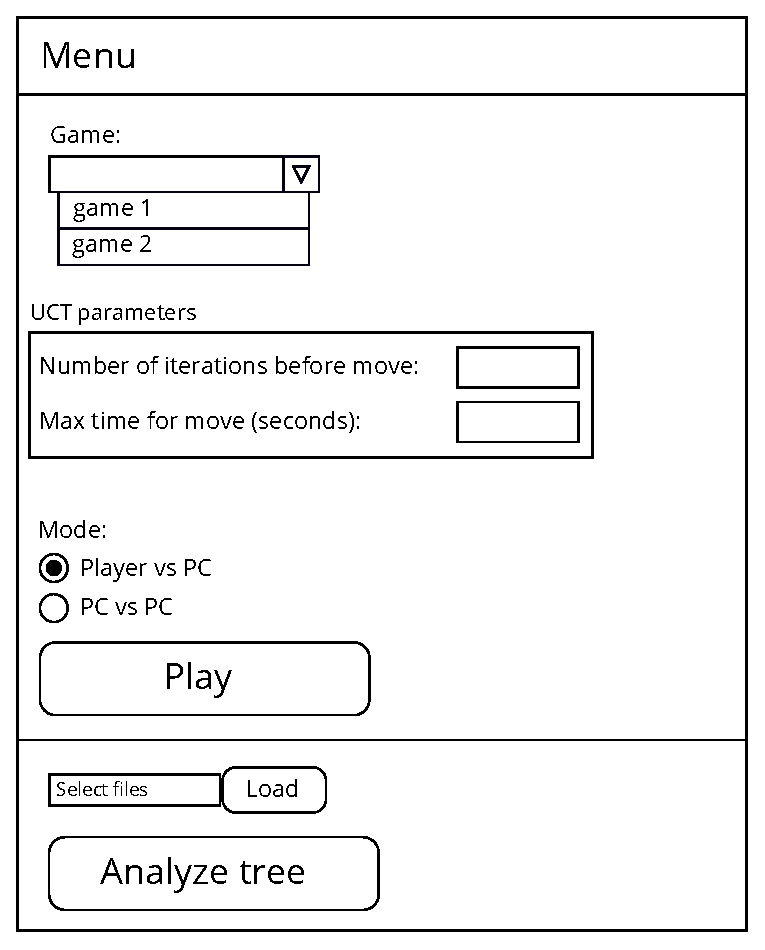
\includegraphics[width=0.4\textwidth]{menu-eps-improved}
	\caption{Okno menu głównego}
	\label{rys:main_menu}
\end{figure}

\noindent Dwa moduły, do których można przejść z tego okna, to rozgrywka i analiza drzewa.	Żeby rozegrać grę, należy nacisnąć na przycisk \textit{Play}. Powyżej tego przycisku znajdować się będzie szereg opcji, który pozwoli użytkownikowi ustawić parametry gry dostosowane do jego preferencji, w tym między innymi:\\

\begin{itemize}
	\item wybór gry - rozwijana lista, w której znajdować się będą zaimplementowane gry (nasz projekt przewiduje dwa tytuły),
	\item liczba iteracji (rozgrywek), jaką komputer będzie wykonywał przed wykonaniem ruchu,
	\item maksymalny czas na wykonanie ruchu - czas, po którym komputer będzie przerywał obliczenia i wykona ruch,
	\item tryb rozgrywki:
	\subitem - człowiek kontra człowiek,
	\subitem - człowiek kontra maszyna,
	\subitem - maszyna kontra maszyna.
\end{itemize}

Analiza drzewa (lub drzew) będzie dostępna po naciśnięciu przycisku \textit{Analyze tree} i uprzedniego wczytania wybranych plików (.tree, .csv).

\subsection{Analiza drzewa}
W oknie ukazanym na rysunku \ref{rys:analyze_tree} będziemy mogli oglądać wczytane lub wygenerowane drzewa. 
\begin{figure}[h!]
	\centering
	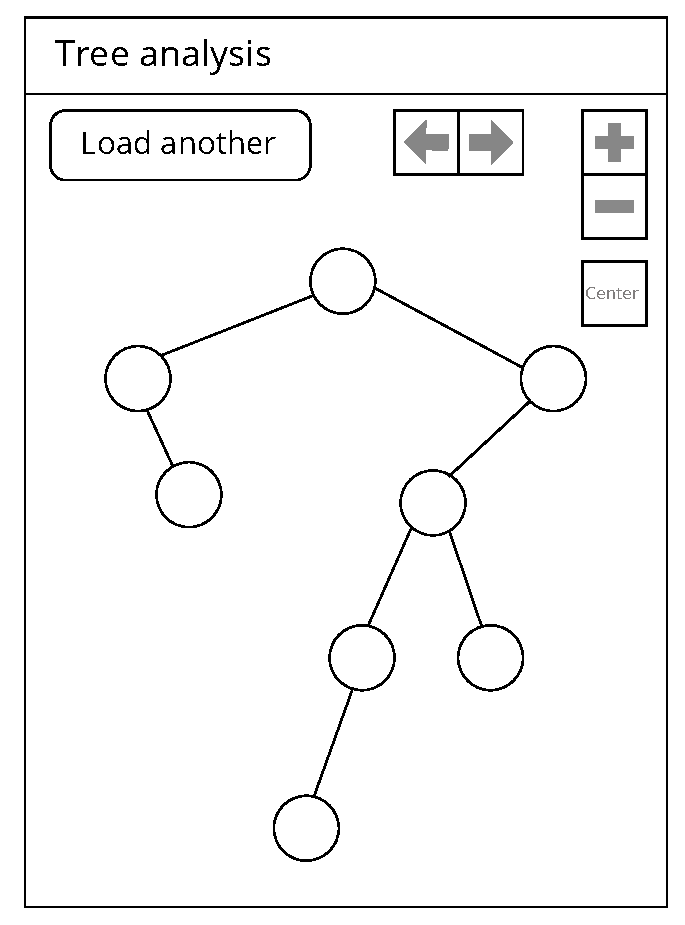
\includegraphics[scale=0.8]{tree-eps-improved}
	\caption{Okno analizy drzewa}
	\label{rys:analyze_tree}
\end{figure}

Kluczową funkcją będzie tutaj możliwość dynamicznego przybliżania i oddalania go (za pomocą przycisków plusa i minusa na ekranie lub scrolla) wraz z możliwością klikania poszczególnych węzłów w celu pozyskania stanu rozgrywki w danym momencie. Widoczna będzie także informacja o tym, ile razy algorytm odwiedził dany węzeł, ile razy doprowadził on do wygranej oraz średnią nagrodę za ruch w danym węźle. Możliwe będzie też wycentrowanie oglądanego drzewa.

W przypadku wczytania większej ilości drzew będzie możliwość przełączania ich za pomocą przycisków ze strzałkami w lewo i w prawo. Zaznaczane wtedy będą różnice w węzłach i krawędziach względem poprzedniego drzewa.

\subsection{Rozgrywka}
Poniżej przedstawiony jest przykładowy interfejs graficzny, do którego użytkownik będzie miał dostęp podczas rozgrywki.
\begin{figure}[h!]
	\centering
	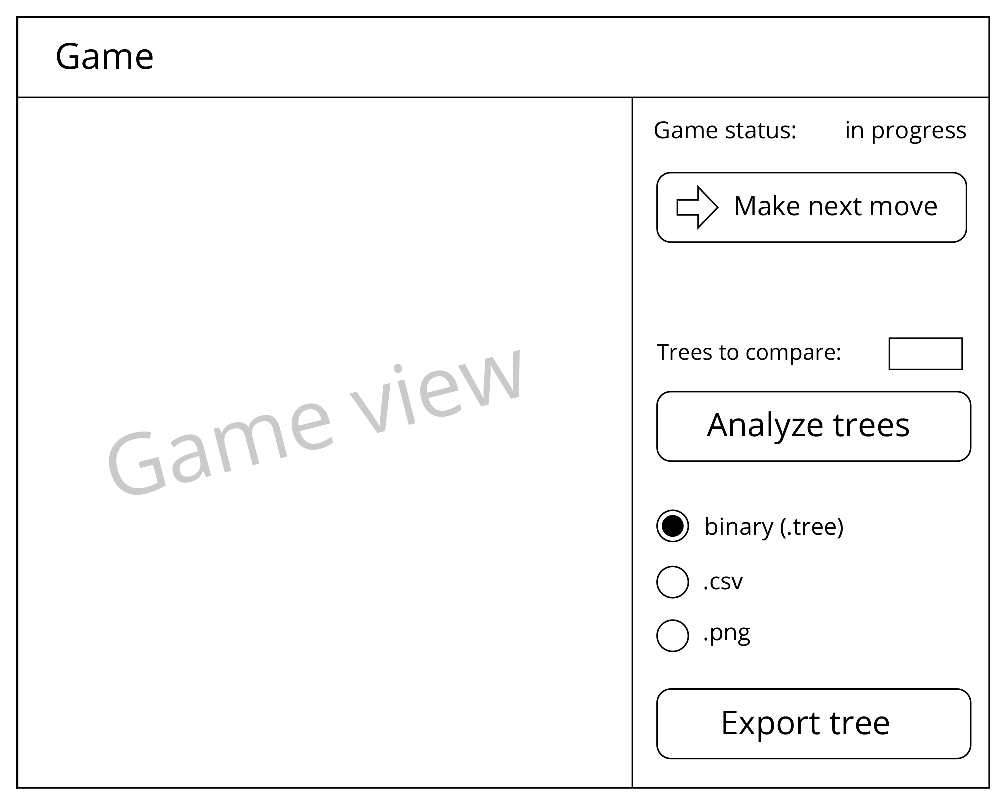
\includegraphics[width=0.7\textwidth]{game-eps-improved}
	\caption{Okno rozgrywki}
	\label{rys:game_view}
\end{figure}

Zgodnie z projektem okna przedstawionym na rysunku \ref{rys:game_view}, widok rozgrywki będzie podzielony na dwie części. Gra zawierać się będzie w wyżej pokazanym oknie po lewej stronie. To tutaj użytkownik za pomocą przygotowanego do gier GUI będzie mógł wykonać ruch. W prawej części okna znajdować się będą opcje związane z aktualnym stanem rozgrywki, między innymi:

\begin{itemize}
	\item informacja o aktualnym stanie gry.
	\item wykonaj kolejny ruch - wyłącznie w trybie rozgrywki maszyna kontra maszyna. Użytkownik będzie miał możliwość kontrolowania wykonywanych przez komputer ruchów, aby samemu móc powodować postęp w rozgrywce.
	\item przeanalizuj wygenerowane drzewa - będzie to przycisk otwierający drugie okno z opisaną wcześniej analizą drzewa. Nad przyciskiem znajduje się parametr mówiący ile ruchów wstecz użytkownik ma zamiar analizować. Jedno drzewo będzie odpowiadać jednemu ruchowi komputera, a jako pierwsze wyświetli się drzewo przedstawiające stan z ostatniego ruchu i reszta będzie odpowiednio w kolejności chronologicznej (od końca).
	\item wyeksportuj drzewo do pliku (csv, png lub binarnego).
\end{itemize}